\documentclass{article}

\usepackage{enumitem}
\usepackage{listings}
\usepackage{color}
\usepackage{amsmath}
\usepackage{hyperref}
\usepackage{graphicx}
\usepackage{pgffor}
\usepackage{xparse}
\usepackage{expl3}
\usepackage{tabularx, makecell}
\usepackage{booktabs}
\usepackage{indentfirst}

\graphicspath{{./}}

\definecolor{codegreen}{rgb}{0,0.6,0}
\definecolor{codegray}{rgb}{0.5,0.5,0.5}
\definecolor{codepurple}{rgb}{0.58,0,0.82}
\definecolor{backcolour}{rgb}{0.95,0.95,0.92}
 
\lstdefinestyle{mystyle}{d
    backgroundcolor=\color{backcolour},   
    commentstyle=\color{codegreen},
    keywordstyle=\color{magenta},
    numberstyle=\tiny\color{codegray},
    stringstyle=\color{codepurple},
    basicstyle=\footnotesize,
    breakatwhitespace=false,         
    breaklines=true,                 
    captionpos=b,                    
    keepspaces=true,                 
    numbers=left,                    
    numbersep=5pt,                  
    showspaces=false,                
    showstringspaces=false,
    showtabs=false,                  
    tabsize=2
}

\begin{document}

	\newcommand{\filePath}[1]{./imgs/#1_graph}
	
	\newcommand{\includegraphicsSized}[1]{
		\includegraphics[scale=0.6]{#1}
	}

	\newcommand{\addLFAGraphImg}[1]{
		\IfFileExists{\filePath{#1}.png}
		{
			\includegraphicsSized{\filePath{#1}.png}
		}
		{
			\includegraphicsSized{\filePath{#1}.jpg}
		}
	}

	\newcommand{\FAState}[3]{
		$\sigma$(#1, #2) = \{#3\}
	}

	\title{LFA laboratory\_01}
	\author{Terman Emil \& Ganuscheak Vlad FAF161}
	\maketitle

	\newpage
	\section{1. Part A}
		$V_N$ = \{S,\ L,\ D\}
		$V_T$ = \{a, b, c, d, e, f, j\}
		\newline
		P = \{
		\newline
		S $\rightarrow$ aS $|$ bS $|$ cD $|$ dL $|$ e
		\newline
		L $\rightarrow$ eL $|$ fL $|$ jD $|$ e
		\newline
		D $\rightarrow$ eD $|$ d
		\}

    \subsection{Presentation of five strings that belong to the language L(G)}
    	\begin{enumerate}
    		\item
    			S $\rightarrow$ dL
    			$\rightarrow$ deL
    			$\rightarrow$ deeL
    			$\rightarrow$ deeeL
    			$\rightarrow$ deeee
				\newline
				\addLFAGraphImg{deeee}

    		\item
    			S $\rightarrow$ aS
    			$\rightarrow$ adL
    			$\rightarrow$ adjD
    			$\rightarrow$ adjeD
    			$\rightarrow$ adjed
    			\newline
				\addLFAGraphImg{adjed}

    		\item
				S $\rightarrow$ cD
				$\rightarrow$ ceD
				$\rightarrow$ ceeD
				$\rightarrow$ ceeeD
				$\rightarrow$ ceeed
				\newline
				\addLFAGraphImg{ceeed}

			\item
				S $\rightarrow$ aS
				$\rightarrow$ aaS
				$\rightarrow$ aadL
				$\rightarrow$ aadjD
				$\rightarrow$ aadjd
				\newline
				\addLFAGraphImg{aadjd}

			\item
				S $\rightarrow$ aS
				$\rightarrow$ abS
				$\rightarrow$ abaS
				$\rightarrow$ abadL
				$\rightarrow$ abadeL
				$\rightarrow$ abadefL
				$\rightarrow$ abadefe
				\newline
				\addLFAGraphImg{abadefe}
    	\end{enumerate}

    	\pagebreak

	\subsection{Conversion of regular grammar to Finite Automaton}
	
		FA = \{Q, $\Sigma$, $\sigma$, S, F\}
		\newline
		Q = \{S, L, D\}
		\newline
		F = \{X\}
		\newline
		$\Sigma$ = \{a, b, c, d, e, f, j\}
		\newline

		\begin{tabular}{m{.40\textwidth}m{.60\textwidth}}
			\toprule
			
			\begin{enumerate}
				\item \FAState{S}{a}{S}
				\item \FAState{S}{b}{S}
				\item \FAState{S}{c}{D}
				\item \FAState{S}{d}{L}
				\item \FAState{S}{e}{X}
				\item \FAState{L}{e}{L}
				\item \FAState{L}{f}{L}
				\item \FAState{L}{j}{D}
				\item \FAState{L}{e}{X}
				\item \FAState{D}{e}{D}
				\item \FAState{D}{d}{X}
			\end{enumerate}
			&
			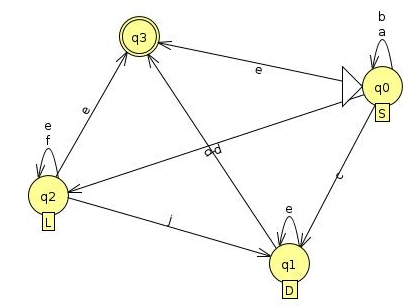
\includegraphics[scale=0.5]{./imgs/FA_graph.jpg}

			\\\bottomrule
		\end{tabular}

	\subsection{Type of the grammar}
			The given grammar is of type 3 - right linear, by Chomsky
		clasifiction, because the productions are only of the type:

		\begin{center}
			\begin{itemize}
				\centering

				\item A $\rightarrow$ xB
				\item A $\rightarrow$ x
			\end{itemize}
		\end{center}

		\pagebreak
\end{document}
